\documentclass[]{article}

% Imported Packages
%------------------------------------------------------------------------------
\usepackage{amssymb}
\usepackage{amstext}
\usepackage{amsthm}
\usepackage{amsmath}
\usepackage{enumerate}
\usepackage{fancyhdr}
\usepackage[margin=1in]{geometry}
\usepackage{graphicx}
\usepackage{float}
\usepackage{placeins}
%\usepackage{extarrows}
%\usepackage{setspace}
%------------------------------------------------------------------------------

% Header and Footer
%------------------------------------------------------------------------------
\pagestyle{plain}  
\renewcommand\headrulewidth{0.4pt}                                      
\renewcommand\footrulewidth{0.4pt}                                    
%------------------------------------------------------------------------------

% Title Details
%------------------------------------------------------------------------------
\title{Deliverable \#2}
\author{SE 3A04: Software Design III -- Large System Design}
\date{}                               
%------------------------------------------------------------------------------

% Document
%------------------------------------------------------------------------------
\begin{document}

\maketitle	
\noindent{\bf Tutorial Number:} T01\\
{\bf Group Number:} G02 \\
{\bf Group Members:} 
\begin{itemize}
	\item Omer Karo
	\item Ahsan Muzammil
	\item Jake Finlay
	\item Ethan Walsh
	\item Rebecca Di Filippo
	\item Abdallah Alqashqish
\end{itemize}

\section*{IMPORTANT NOTES}
\begin{itemize}
	%	\item You do \underline{NOT} need to provide a text explanation of each diagram; the diagram should speak for itself
	\item Please document any non-standard notations that you may have used
	\begin{itemize}
		\item \emph{Rule of Thumb}: if you feel there is any doubt surrounding the meaning of your notations, document them
	\end{itemize}
	\item Some diagrams may be difficult to fit into one page
	\begin{itemize}
		\item Ensure that the text is readable when printed, or when viewed at 100\% on a regular laptop-sized screen.
		\item If you need to break a diagram onto multiple pages, please adopt a system of doing so and thoroughly explain how it can be reconnected from one page to the next; if you are unsure about this, please ask about it
	\end{itemize}
	\item Please submit the latest version of Deliverable 1 with Deliverable 2
	\begin{itemize}
		\item Indicate any changes you made.
	\end{itemize}
	\item If you do \underline{NOT} have a Division of Labour sheet, your deliverable will \underline{NOT} be marked
\end{itemize}

\newpage
\section{Introduction}
\label{sec:introduction}
% Begin Section

This section should provide an brief overview of the entire document.

\subsection{Purpose}
\label{sub:purpose}
% Begin SubSection
This document provides a high level overview of the DealCheck system architecture, including high level design considerations of the system, as well as design considerations for various subsystems. This document is intended for internal DealCheck stakeholders, including project managers, software developers, domain experts, and DealCheck team members/investors. It is recommended that DealCheck deliverable 1 is read prior, and the reader has some basic software technical knowledge.
% End SubSection

\subsection{System Description}
\label{sub:system_description}
% Begin SubSection
The overall DealCheck system follows a Blackboard (BB) style architecture, with various subsystems adopting either a BB or repository style design architecture.
The BB architecture supports multiple agents or "experts" that contribute toward the evaluation of car deals, with each agent operating independently to add insights to the shared Blackboard, which acts as the central repository of knowledge.
Additionally, the repository style design architecture is used for subsystems that require concurrent access to data, particularly in areas like account management. This architecture is specialized for handling high-complexity data processing, ensuring that user account information and car evaluation reports are securely and efficiently managed in DealCheck.
% End SubSection

\subsection{Overview}
\label{sub:overview}
% Begin SubSection
Section 2 presents an Analysis Class Diagram. In Section 3, the document goes into the architectural design of the system, as well as discusses considered alternatives, and reasoning behind design decisions. Next, in Section 4, Class Responsibility Collaboration (CRC) Cards are presented to understand the inside of the classes, their responsibilities, and the interactions between classes. Lastly Section A, is the division of labour section where we discuss who focused on which parts.

% End SubSection

% End Section

\section{Analysis Class Diagram}
\label{sec:analysis_class_diagram}
% Begin Section
\begin{figure}[H]
	\centering
	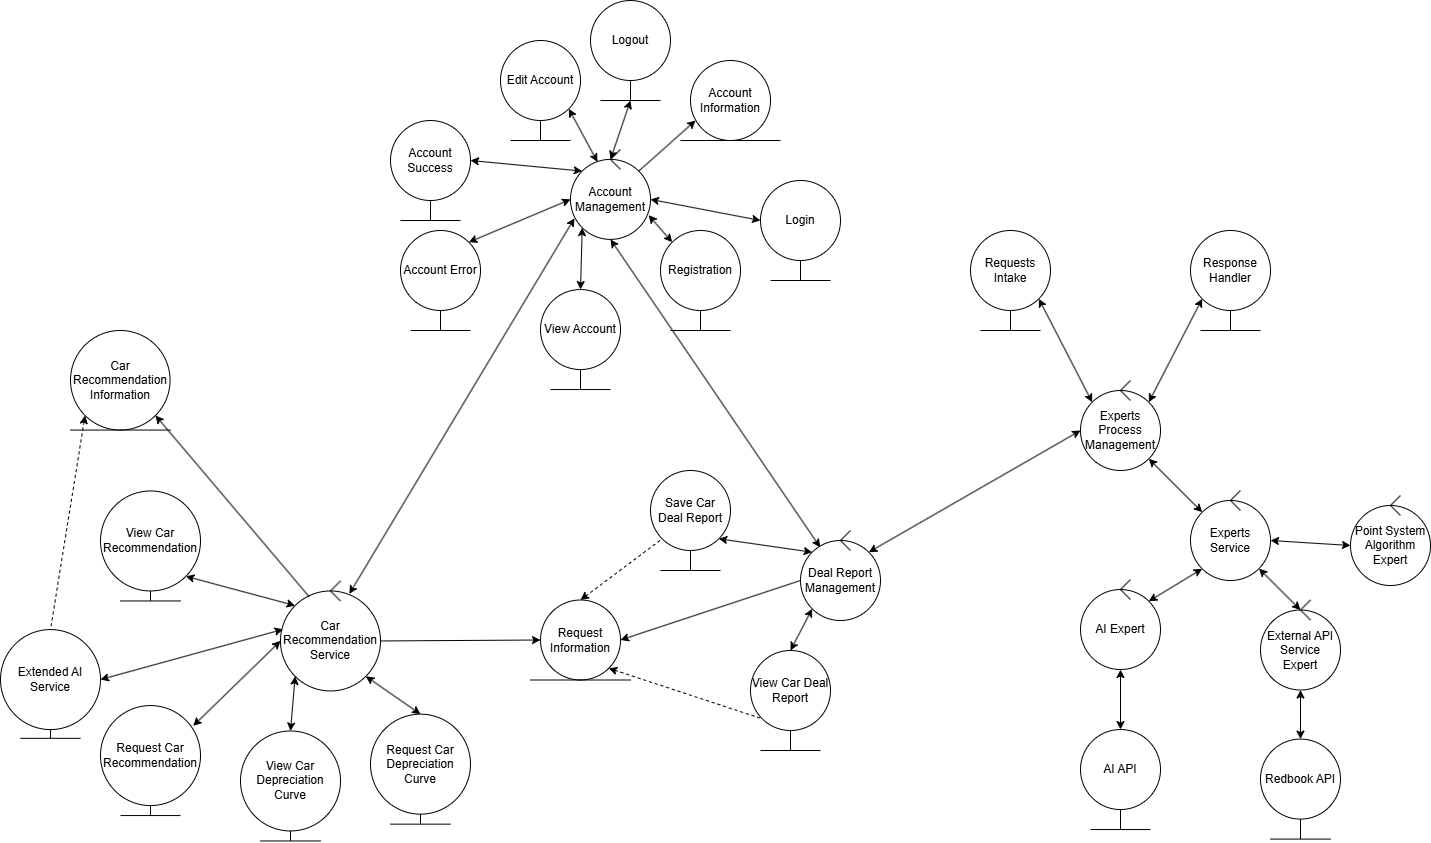
\includegraphics[scale=0.35]{3A04_acd.png}
	\caption{Analysis Class Diagram}\label{Fig:2.1}
\end{figure}
% End Section


\section{Architectural Design}
\label{sec:architectural_design}
% Begin Section
This section should provide an overview of the overall architectural design of your application. Your overall architecture should show the division of the system into subsystems with high cohesion and low coupling.

\subsection{System Architecture}

\begin{figure}[H]
	\centering
	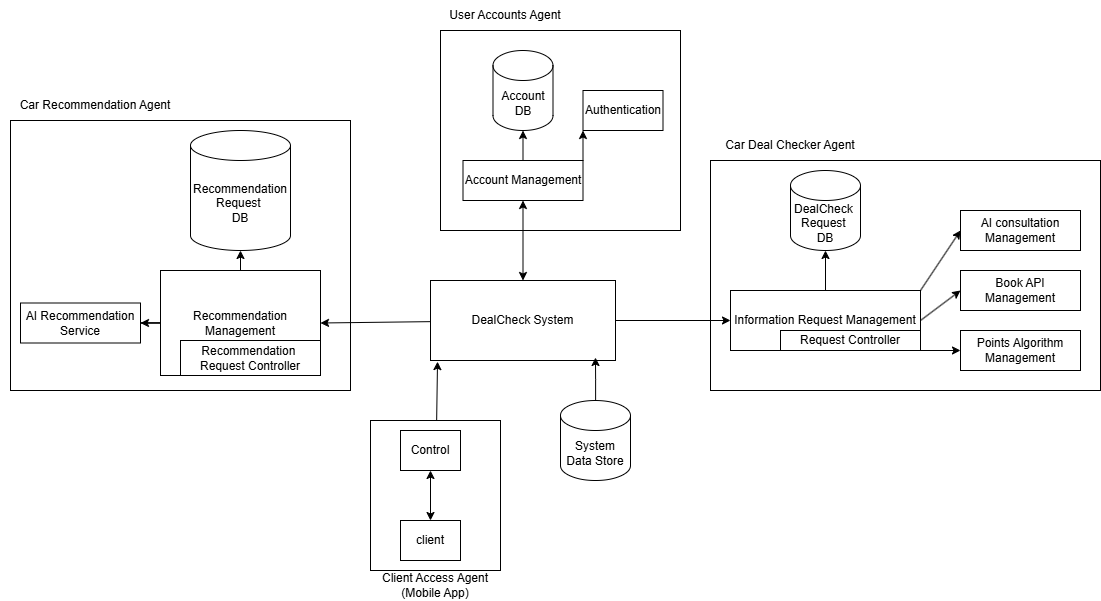
\includegraphics[scale=0.45]{3A04_sys2.png}
	\caption{System Diagram}\label{Fig:2.1}
\end{figure}

\label{sub:system_architecture}
% Begin SubSection
\begin{itemize}
	\item Identify and explain the overall architecture of your system
	\item Be sure to clearly state the name of the architecture you used (this is the name of the architectural pattern, not the name of your system)
	\item Provide the reasoning and justification of the choice of architecture
	\item Provide a structural architecture diagram showing the relationship among the subsystems (if appropriate)
	\item List any design alternatives you considered, but eliminated (and explain why you eliminated them)
\end{itemize}

DealCheck will utilize a Data-Centered architecture, namely the Blackboard architecture style. The system's core functionality is accessed through the System Controller via the Client Access Agent. The Client Access Agent will control the user interface of the application. The System Controller will act as the central ‘data store’ used in Blackboard architecture, while each of the subsystems described below will act as the ‘knowledge sources.’ These include the Car Recommendation Agent, the User Accounts Agent, and the Car Deal Checker Agent. \\

The following table summarizes the purpose and architectural style of each subsystem:
\FloatBarrier
\begin{table}[H]
    \centering
    \begin{tabular}{|p{4cm}|p{7cm}|p{3cm}|}
        \hline
        \textbf{Subsystem} & \textbf{Purpose} & \textbf{Architectural Style} \\
        \hline
        Account Management & Users manage, modify, and create account-related data. & Repository \\
        \hline
        Deal Report Management & Users query the system for information on a car deal as well as view and save results. & Blackboard \\
        \hline
        Recommendation Management & Users obtain recommendations on car purchases. & Blackboard \\
        \hline
    \end{tabular}
    \label{tab:dealcheck_subsystems}
\end{table}
\FloatBarrier
\noindent
Further subsystem descriptions are provided in Section 3.2 of this document. \\
\newline
This system will also employ four databases:
\begin{itemize}
    \item The \textbf{Account Database} will hold user information such as usernames and passwords.
    \item The \textbf{Recommendation Request Database} and \textbf{DealCheck Request Database} will store records from user queries in their respective systems.
    \item The \textbf{System Data Store} will act as the central data store for the entire application.
\end{itemize}

DealCheck's architecture utilizes both the Repository and Blackboard systems. The overall system employs the Blackboard architecture since it enables separation of application components (as shown in Table \ref{tab:dealcheck_subsystems}), allowing them to function independently. The system data store also houses application-wide data, including user interface details and request information. This central data store invokes the correct subsystems based on the request. \\

Blackboard is particularly suitable for the information request management subsystem because vehicle valuation lacks a single correct answer. Multiple knowledge sources must be consulted and integrated to generate a high-quality response. This aligns with the Blackboard style, where the data store is active and calls upon relevant knowledge sources to process a query. The Blackboard approach was preferred over Batch Sequential and Repository due to the non-deterministic nature of vehicle deal evaluations, which benefit from multiple consulted agents. \\

The Repository architecture is employed for the Account Management system, as it is commonly used in database management applications requiring frequent data modifications. Unlike the Blackboard system, which actively calls knowledge sources, the Repository architecture features a passive data store, making it ideal for account management tasks performed by users. Other data-centered architectures like Blackboard were unsuitable because account management does not involve solving non-deterministic problems. Data Flow architectures were also not selected, as this system does not rely on sequential data transformations. The Repository model's key strength is ensuring data integrity, which is essential for securing sensitive user information such as usernames and passwords. \\

We considered the Batch Sequential approach from the Data Flow architecture to handle car deal requests, where a user submits a request and DealCheck processes it through the Deal Report Management system. However, this approach was unsuitable because the system requires real-time responses, whereas batch processing introduces delays. Users expect instant feedback on deal evaluations, making batch cycles impractical. Furthermore, Batch Sequential has low throughput due to its rigid, sequential steps, making it inefficient for a multi-user application. \\

Another alternative explored was Pipes and Filters for the Deal Report Management subsystem. However, this architecture lacks the flexibility required for non-deterministic car deal evaluations. Different deals may require varying types of analysis depending on user input and consulted experts, making a fixed sequence of processing steps suboptimal. Pipes and Filters work best for structured data transformations, whereas DealCheck's subsystems require dynamic data integration from multiple sources, making this architecture unsuitable. \\

We also considered the Process-Control architecture but ultimately eliminated it because it is designed for continuous monitoring and real-time feedback loops, such as temperature regulation systems. DealCheck, however, operates on user-initiated queries rather than ongoing system monitoring, making Process-Control unnecessary for this application. \\

% End SubSection

\subsection{Subsystems}
\label{sub:subsystems}
% Begin SubSection
Provide a list of your subsystems, with a brief description of each. Be sure to document its purpose and relationship to other subsystems.

Dealcheck’s primary system has been subdivided into three subsystems: Account Management, Deal Report Management, and Car Recommendation Service. \\

Account Management will serve as the center for all related information and queries to account details. This will include storing information such as usernames and passwords. Functions of this system will primarily be for modification of this information, for example, a function to reset a user’s password. \\

The Deal Report Management subsystem serves as the core functionality of the DealCheck app, enabling users to view previous car deal reports, save new reports, and request car deal evaluations. It interacts with the Account Management subsystem to retrieve a user's past queries by linking their account information with the app's query history. Additionally, it interacts with the Account Management subsystem to save car deal reports to the corresponding user accounts. This subsystem also handles car deal evaluation requests, collaborating with controllers like Experts Process Management to process requests, select the appropriate experts based on user input, and generate detailed car deal reports. Finally, this subsystem saves the results of the user's car deal evaluation request in its request information entity, which acts as a gateway to its database. \\

The Car Recommendation Service subsystem is our innovative feature, responsible for handling user requests related to car recommendations and depreciation curves, displaying results, and generating these insights. It collaborates with the Account Management subsystem to authenticate users and grant access to its functionalities. When a user requests car recommendations based on their specific scenario, the subsystem uses an Extended AI Service to generate personalized suggestions. Additionally, it stores AI-generated car recommendations in the car recommendation information entity, which serves as a gateway to its database. The subsystem also leverages the request information entity within the Deal Report Management subsystem to access past car deal reports, track previously evaluated vehicles, generate depreciation curves, and link them to the corresponding car deals.

% End SubSection

% End Section
	
\section{Class Responsibility Collaboration (CRC) Cards}
\label{sec:class_responsibility_collaboration_crc_cards}
% Begin Section
This section should contain all of your CRC cards.

\begin{itemize}
	\item Provide a CRC Card for each identified class
	\item Please use the format outlined in tutorial, i.e., 
	\begin{table}[H]
		\centering
		\begin{tabular}{|p{6cm}|p{6cm}|}
		\hline 
		 \multicolumn{2}{|l|}{\textbf{Class Name:}} \\
		\hline
		\textbf{Responsibility:} & \textbf{Collaborators:} \\
		\hline
		\vspace{1in} & \\
		\hline
		\end{tabular}
	\end{table}
        \begin{table}[H]
            \centering
            \begin{tabular}{|p{6cm}|p{6cm}|}
            \hline 
          \multicolumn{2}{|l|}{\textbf{Class Name: Registration (Boundary)}} \\
            \hline
            \textbf{Responsibility:} & \textbf{Collaborators:} \\
            \hline
               Handles click-event on “Make New Profile” button & Account        Management Controller \\
                 Knows Account Management Controller &\\
            \hline
            \end{tabular}
        \end{table}
        \begin{table}[H]
            \centering
            \begin{tabular}{|p{6cm}|p{6cm}|}
            \hline 
             \multicolumn{2}{|l|}{\textbf{Class Name: Login (Boundary)}} \\
            \hline
            \textbf{Responsibility:} & \textbf{Collaborators:} \\
            \hline
            Handles click-event on “Login” button &  Account Management Controller \\
                Knows Account Management Controller & \\
            \hline
            \end{tabular}
        \end{table}
        \begin{table}[H]
            \centering
            \begin{tabular}{|p{6cm}|p{6cm}|}
            \hline 
             \multicolumn{2}{|l|}{\textbf{Class Name: Account Information (Entity)}} \\
            \hline
            \textbf{Responsibility:} & \textbf{Collaborators:} \\
            \hline
            Knows Account Management Controller & Account Management Controller\\ 
                 Stores account information (i.e username,email,etc.) & \\
            \hline
            \end{tabular}
        \end{table}
        \begin{table}[H]
            \centering
            \begin{tabular}{|p{6cm}|p{6cm}|}
            \hline 
             \multicolumn{2}{|l|}{\textbf{Class Name: View Account (Boundary)}} \\
            \hline
            \textbf{Responsibility:} & \textbf{Collaborators:} \\
            \hline
            Handles click-event on “View Profile” button & Account Management Controller\\
            Displays Account Information &  \\
                Knows Account Managment Controller &  \\
            \hline
            \end{tabular}
        \end{table}
        \begin{table}[H]
            \centering
            \begin{tabular}{|p{6cm}|p{6cm}|}
            \hline 
             \multicolumn{2}{|l|}{\textbf{Class Name: Experts Service (Controller)}} \\
            \hline
            \textbf{Responsibility:} & \textbf{Collaborators:} \\
            \hline
            Knows Experts Process Management Controller & Experts Process Management \\
            Knows AI Expert & AI Expert \\
            Knows External API Service Expert & External API Service Expert \\
            Knows Point System Algorithm Expert & Point System Algorithm Expert \\
            Handles interaction between the process manager and the experts & \\
            \hline
            \end{tabular}
        \end{table}
        \begin{table}[H]
            \centering
            \begin{tabular}{|p{6cm}|p{6cm}|}
            \hline 
             \multicolumn{2}{|l|}{\textbf{Class Name: AI Expert (Controller)}} \\
            \hline
            \textbf{Responsibility:} & \textbf{Collaborators:} \\
            \hline
            Knows Experts Service & Experts Service \\
            Knows AI API & AI API \\
            Processes AI queries & \\
            \hline
            \end{tabular}
        \end{table}     
        \begin{table}[H]
            \centering
            \begin{tabular}{|p{6cm}|p{6cm}|}
            \hline 
             \multicolumn{2}{|l|}{\textbf{Class Name: AI API (Boundary)}} \\
            \hline
            \textbf{Responsibility:} & \textbf{Collaborators:} \\
            \hline
            Knows AI Expert & AI Expert \\
            Handles AI queries & \\
            \hline
            \end{tabular}
        \end{table}
        \begin{table}[H]
            \centering
            \begin{tabular}{|p{6cm}|p{6cm}|}
            \hline 
             \multicolumn{2}{|l|}{\textbf{Class Name: External API Service Expert (Controller)}} \\
            \hline
            \textbf{Responsibility:} & \textbf{Collaborators:} \\
            \hline
            Knows Experts Service & Experts Service \\
            Knows Redbook API & Redbook API \\
            Processes external API requests & \\
            \hline
            \end{tabular}
        \end{table}  
        \begin{table}[H]
            \centering
            \begin{tabular}{|p{6cm}|p{6cm}|}
            \hline 
             \multicolumn{2}{|l|}{\textbf{Class Name: Redbook API (Boundary)}} \\
            \hline
            \textbf{Responsibility:} & \textbf{Collaborators:} \\
            \hline
            Knows External API Service Expert & External API Service Expert \\
            Handles requests to the Redbook API & \\
            \hline
            \end{tabular}
        \end{table}
        \begin{table}[H]
            \centering
            \begin{tabular}{|p{6cm}|p{6cm}|}
            \hline 
             \multicolumn{2}{|l|}{\textbf{Class Name: Point System Algorithm (Controller)}} \\
            \hline
            \textbf{Responsibility:} & \textbf{Collaborators:} \\
            \hline
            Knows Experts Service & Experts Service \\
            Handles point calculations & \\
            \hline
            \end{tabular}
        \end{table}
        \begin{table}[H]
            \centering
            \begin{tabular}{|p{6cm}|p{6cm}|}
            \hline 
             \multicolumn{2}{|l|}{\textbf{Class Name: Deal Report Management (Controller)}} \\
            \hline
            \textbf{Responsibility:} & \textbf{Collaborators:} \\
            \hline
            Knows Account Management & Account Management \\
            Knows Experts Process Management & Experts Process Management \\
            Knows Request Information & Request Information \\
            Knows View Car Deal Report & View Car Deal Report \\
            Knows Save Car Deal Report & Save Car Deal Report \\
            Handles deal reports & \\
            \hline
            \end{tabular}
        \end{table}
        \begin{table}[H]
            \centering
            \begin{tabular}{|p{6cm}|p{6cm}|}
            \hline 
             \multicolumn{2}{|l|}{\textbf{Class Name: View Car Deal Report (Boundary)}} \\
            \hline
            \textbf{Responsibility:} & \textbf{Collaborators:} \\
            \hline
            Knows Request Information & Request Information \\
            Knows Deal Report Management & Deal Report Management \\
            Handles click event of “View Deal Report” & \\
            Displays deal report information & \\
            \hline
            \end{tabular}
        \end{table}   
        \begin{table}[H]
            \centering
            \begin{tabular}{|p{6cm}|p{6cm}|}
            \hline 
             \multicolumn{2}{|l|}{\textbf{Class Name: Save Car Deal Report (Boundary)}} \\
            \hline
            \textbf{Responsibility:} & \textbf{Collaborators:} \\
            \hline
            Knows Request Information & Request Information \\
            Knows Deal Report Management & Deal Report Management \\
            Handles click event of “Save Deal Report” & \\
            Saves deal report information & \\
            \hline
            \end{tabular}
        \end{table}
        \begin{table}[H]
            \centering
            \begin{tabular}{|p{6cm}|p{6cm}|}
                \hline 
                \multicolumn{2}{|l|}{\textbf{Class Name: Requests Intake (Boundary)}} \\
                \hline
                \textbf{Responsibility:} & \textbf{Collaborators:} \\
                \hline
                Handles deal valuation requests & Experts Process Manager \\
                \hline
            \end{tabular}
        \end{table}
        \begin{table}[H]
            \centering
            \begin{tabular}{|p{6cm}|p{6cm}|}
                \hline 
                \multicolumn{2}{|l|}{\textbf{Class Name: Response Handler (Boundary)}} \\
                \hline
                \textbf{Responsibility:} & \textbf{Collaborators:} \\
                \hline
                Handles deal valuation responses & Experts Process Manager \\
                \hline
            \end{tabular}
        \end{table}
        \begin{table}[H]
            \centering
            \begin{tabular}{|p{6cm}|p{6cm}|}
                \hline 
                \multicolumn{2}{|l|}{\textbf{Class Name: Car Recommendation Service (Controller)}} \\
                \hline
                \textbf{Responsibility:} & \textbf{Collaborators:} \\
                \hline
                \text{Knows Account Management} & Account Management \\
                Knows View Car Recommendation & View Car Recommendation \\
                Knows Request Car Depreciation Curve & Request Car Depreciation Curve \\
                Knows View Car Depreciation Curve & View Car Depreciation Curve \\
                Knows AI Car Recommendation service & AI Car Recommendation service \\
                Knows Car Recommendation Information & Car Recommendation Information \\
                Knows Request Information & Request Information \\
                Handles Car Recommendations Requests &  \\
                Handles Car Depreciation Curve Requests &  \\
                \hline
            \end{tabular}
        \end{table}
        \begin{table}[H]
            \centering
            \begin{tabular}{|p{6cm}|p{6cm}|}
                \hline 
                \multicolumn{2}{|l|}{\textbf{Class Name: Request Car Depreciation Curve (Controller)}} \\
                \hline
                \textbf{Responsibility:} & \textbf{Collaborators:} \\
                \hline
                Handles Car Depreciation Curve Requests From External AI & Car Recommendation Service \\
                \hline
            \end{tabular}
        \end{table}
        \begin{table}[H]
            \centering
            \begin{tabular}{|p{6cm}|p{6cm}|}
            \hline 
             \multicolumn{2}{|c|}{\textbf{Class Name: Car Recommendation Information (Entity)}} \\
            \hline
            \textbf{Responsibility} & \textbf{Collaborators} \\
            \hline
            Know the car recommendation database & Car Recommendation Service \\
            Process the interaction with car recommendation database & AI Car Recommendation Service \\
            Process the data interaction with car recommendation service & \\
            \hline
            \end{tabular}
        \end{table}
        \begin{table}[H]
            \centering
            \begin{tabular}{|p{6cm}|p{6cm}|}
            \hline 
             \multicolumn{2}{|c|}{\textbf{Class Name: Account Management (Controller)}} \\
            \hline
            \textbf{Responsibility} & \textbf{Collaborators} \\
            \hline
            Knows user account information & Edit Account\\
            Processes user authentication requests (login, logout, registration) & Account Success\\
            Processes user data requests (view, edit) & Account Error\\
            Handles account error handling & View Account\\
            & Account Information \\
            & Registration\\
            & Login\\
            & Logout\\
            \hline
            \end{tabular}
        \end{table}
        \begin{table}[H]
            \centering
            \begin{tabular}{|p{6cm}|p{6cm}|}
            \hline 
             \multicolumn{2}{|c|}{\textbf{Class Name: Logout (Boundary)}} \\
            \hline
            \textbf{Responsibility} & \textbf{Collaborators} \\
            \hline
            Knows user account information & Account Management\\
            Processes logout requests by the user & \\
            \hline
            \end{tabular}
        \end{table}
        \begin{table}[H]
            \centering
            \begin{tabular}{|p{6cm}|p{6cm}|}
            \hline 
             \multicolumn{2}{|c|}{\textbf{Class Name: Account Success (Boundary)}} \\
            \hline
            \textbf{Responsibility} & \textbf{Collaborators} \\
            \hline
            Knows user account information & Account Management\\
            Handles successful user account interactions (successful login/logout/registration) & \\
            \hline
            \end{tabular}
        \end{table}
        \begin{table}[H]
            \centering
            \renewcommand{\arraystretch}{1.3} % Increases row height for better readability
            \begin{tabular}{|p{6cm}|p{6cm}|} 
            \hline
            \multicolumn{2}{|c|}{\textbf{Class Name: View Car Depreciation Curve (Boundary)}} \\ 
            \hline
            \textbf{Responsibility} & \textbf{Collaborators} \\ 
            \hline
            Handles click-event on "View Depreciation Curve" \newline
            Knows Car Recommendation Service Controller \newline
            Displays Car Depreciation Curve & Car Recommendation Service Controller \\ 
            \hline
            \end{tabular}
        \label{tab:crc_card}
        \end{table}   
        \begin{table}[H]
            \centering
            \renewcommand{\arraystretch}{1.3} % Increases row height for better readability
            \begin{tabular}{|p{6cm}|p{6cm}|} 
            \hline
            \multicolumn{2}{|c|}{\textbf{Class Name: Request Car Recommendation (Boundary)}} \\ 
            \hline
            \textbf{Responsibility} & \textbf{Collaborators} \\ 
            \hline
            Handle scenario-based car recommendation request \newline
            Knows Car Recommendation Service Controller \newline
            Implicit request from external AI Car Recommendation Service & Car Recommendation Service Controller \\ 
            \hline
            \end{tabular}
            \label{tab:crc_card}
        \end{table}
            
        \begin{table}[H]
        \centering
        \renewcommand{\arraystretch}{1.3} % Increases row height for better readability
        \begin{tabular}{|p{6cm}|p{6cm}|} 
        \hline
        \multicolumn{2}{|c|}{\textbf{Class Name: View Car Recommendation (Boundary)}} \\ 
        \hline
        \textbf{Responsibility} & \textbf{Collaborators} \\ 
        \hline
        Handles click-event on “View Recommendation” \newline
        Knows Car Recommendation Service Controller \newline
        Displays Car Recommendation based on user scenario & Car Recommendation Service Controller \\ 
        \hline
        \end{tabular}
        \label{tab:crc_card}
        \end{table}
            
        \begin{table}[H]
        \centering
        \renewcommand{\arraystretch}{1.3} % Increases row height for better readability
        \begin{tabular}{|p{6cm}|p{6cm}|} 
        \hline
        \multicolumn{2}{|c|}{\textbf{Class Name: AI Car Recommendation Service (Boundary)}} \\ 
        \hline
        \textbf{Responsibility} & \textbf{Collaborators} \\ 
        \hline
        Knows Car Recommendation Service Controller \newline
        Handles AI car recommendation queries based on user scenario & Car Recommendation Service Controller \\ 
        \hline
        \end{tabular}
        \label{tab:crc_card}
        \end{table}

        \begin{table}[H]
        \centering
        \renewcommand{\arraystretch}{1.3} % Increases row height for better readability
        \begin{tabular}{|p{6cm}|p{6cm}|} 
        \hline
        \multicolumn{2}{|c|}{\textbf{Class Name: Request Information (Entity)}} \\ 
        \hline
        \textbf{Responsibility} & \textbf{Collaborators} \\ 
        \hline
        Knows Request Database & View Car Deal Report \\
        Knows Car Deal Report & Save Car Deal Report \\
        Knows Car Recommendations & Car Recommendation Service \\
        \hline
        \end{tabular}
        \label{tab:crc_card}
        \end{table}

        \begin{table}[H]
        \centering
        \renewcommand{\arraystretch}{1.3} % Increases row height for better readability
        \begin{tabular}{|p{6cm}|p{6cm}|} 
        \hline
        \multicolumn{2}{|c|}{\textbf{Class Name: Experts Process Management (Controller}} \\ 
        \hline
        \textbf{Responsibility} & \textbf{Collaborators} \\ 
        \hline
        Knows the status of expert decisions & Experts Service \\
        Knows the results of expert decisions & Response Handler \\ 
        Knows deal report management controller & Requests Intake \\
        Knows expert service controller & \\
        Knows list of requests& \\
        Knows Request Database & \\
        \hline
        \end{tabular}
        \label{tab:crc_card}
        \end{table}

        \begin{table}[H]
        \centering
        \renewcommand{\arraystretch}{1.3} % Increases row height for better readability
        \begin{tabular}{|p{6cm}|p{6cm}|} 
        \hline
        \multicolumn{2}{|c|}{\textbf{Class Name: Account Error (Boundary)}} \\ 
        \hline
        \textbf{Responsibility} & \textbf{Collaborators} \\ 
        \hline
        Handles login error events & Account Management \\
        Handles password error events & \\
        Handles data security error events & \\
        Knows routines to notify the user of the error(s) & \\
        Knows account management controller & \\
        \hline
        \end{tabular}
        \label{tab:crc_card}
        \end{table}

        \begin{table}[H]
        \centering
        \renewcommand{\arraystretch}{1.3} % Increases row height for better readability
        \begin{tabular}{|p{6cm}|p{6cm}|} 
        \hline
        \multicolumn{2}{|c|}{\textbf{Class Name: Request Information (Boundary)}} \\ 
        \hline
        \textbf{Responsibility} & \textbf{Collaborators} \\ 
        \hline
        Handles click-event on "Edit Profile" button & Account Management \\
        Knows Account Management Controller & \\
        Knows which profile fields are modifiable & \\
        \hline
        \end{tabular}
        \label{tab:crc_card}
        \end{table}
\end{itemize}
% End Section

\appendix
\section{Division of Labour}
\label{sec:division_of_labour}
% Begin Section
\subsection{Ahsan Muzammil}
\begin{itemize}
    \item Section 3.1: Wrote about the different architecture designs we considered but eliminated.
    \item Section 3.2: Wrote about each subsystem and how they interact with each other.
    \item \textbf{Class Responsibility Cards:} Contributed to four CRC cards:
    \begin{itemize}
        \item View Car Depreciation Curve
        \item Request Car Recommendation
        \item AI Car Recommendation Service
        \item View Car Recommendation
    \end{itemize}
    \item Suggested changes to the Analysis Class Diagram.
    \begin{center}
        
\includegraphics[scale=0.1]{ahsan.jpeg}
    \end{center}
\end{itemize}

\subsection{Rebecca Di Filippo}
\begin{itemize}
    \item Wrote Section 1.1: Purpose of Document
    \item Wrote Section 1.2: System Description
    \item Wrote Section 1.3: Overview of Document
    \item Contributed 4 Class Responsibility Cards
    \begin{itemize}
        \item Registration
        \item Login
        \item Account Information
        \item View Account
    \end{itemize}
    \begin{center}
        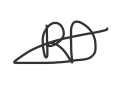
\includegraphics[scale=0.7]{rebecca.png}
    \end{center}
\end{itemize}

\subsection{Ethan Walsh}
\begin{itemize}
    \item Section 3: Derived initial system diagram.
    \item Section 3: Proposed edits to updated system diagram.
    \item Section 3: Wrote initial description of system architecture
    \item Section 3: Wrote description of used architecture styles and rationale
    \item Section 3: Wrote part of section 3.2, Subsystems
    \item Contributed 4 Class Responsibility Cards
    \begin{itemize}
        \item Experts Process Management
        \item Edit Account
        \item Request Information
        \item Account Error
    \end{itemize}
    \begin{center}
        
\includegraphics[scale=0.7]{ethan.png}
    \end{center}
\end{itemize}

\subsection{Jake Finlay}
\begin{itemize}
    \item Came up with some classes for the initial Analysis Class Diagram
    \item Contributed 9 Class Responsibility Cards
    \begin{itemize}
        \item Experts Service
        \item Point System Algorithm Expert
        \item External API Service Expert
        \item Redbook API
        \item AI Expert
        \item AI API
        \item Deal Report Management
        \item View Car Deal Report
        \item Save Car Deal Report
    \end{itemize}
    \item Helped with conversion to Latex
    \begin{center}
        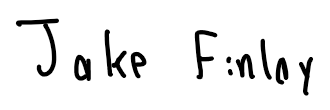
\includegraphics[scale=0.7]{jake.png}
    \end{center}
\end{itemize}

\subsection{Omer Karo}
\begin{itemize}
    \item created initial analysis class diagram for the car recommendation service subsystem
    \item created initial analysis class diagram for the deal report management subsystem
    \item created initial analysis class diagram for the experts process management
    \item Contributed 4 Class Responsibility Cards
    \begin{itemize}
        \item Request Intake
        \item Response Handler
        \item Car Recommendation service
        \item Request Car Depreciation Curve 
    \end{itemize}
    \begin{center}
        
\includegraphics[scale=0.1]{omer.jpg}
    \end{center}
    \item Helped with conversion to Latex
\end{itemize}

\subsection{Abdallah Alqashqish}
\begin{itemize}
    \item Section 2: Collaborated on the Analysis Class Diagram (created and determined initial functionality of)
        \begin{itemize}
            \item Account Management Controller.
            \item Experts service.
            \item Refactored experts that depend on API to use a controller and boundary.
        \end{itemize}
    \item Section 3.1: Refined system architecture diagram to match the final agreed upon architecture.
    \item Contributed 4 Class Responsibility Cards
        \begin{itemize}
            \item Car Recommendation Information (Entity).
            \item Account Management (Controller).
            \item Logout (Boundary).
            \item Account Success (Boundary).
        \end{itemize}
    \item Reviewed Class Responsibility Cards to ensure that they match Analysis Class Diagram.
    \begin{center}
        
\includegraphics[scale=0.1]{abdallah.jpg}
    \end{center}
\end{itemize}
% End Section


\end{document}
%------------------------------------------------------------------------------